% Supporting_Information.tex

\documentclass[11pt]{article}
\usepackage{graphicx}
\bibliographystyle{unsrt}
\usepackage{amsmath}
\usepackage{hyperref}
\usepackage{lipsum}
\usepackage{soul}
\usepackage{url}
\usepackage{multirow}
\usepackage{booktabs}
\usepackage{siunitx}
\usepackage{float} 
\usepackage{placeins}
\usepackage{fancyhdr}
\usepackage[margin=1in]{geometry}
\usepackage{setspace}
\setstretch{1.05}
\setlength{\parindent}{0pt}



% Make numbering S1, S2…
\newcommand{\beginsupplement}{
    \setcounter{table}{0}
    \renewcommand{\thetable}{S\arabic{table}}
    \setcounter{figure}{0}
    \renewcommand{\thefigure}{S\arabic{figure}}
}


\begin{document}
\renewcommand{\thepage}{S-\arabic{page}}

\pagestyle{fancy}
\fancyhf{}                  % clear all header/footer
\fancyhead[R]{\thepage}     % page number top right
\renewcommand{\headrulewidth}{0pt}  % remove header line
\renewcommand{\footrulewidth}{0pt}
\beginsupplement

\renewcommand\figurename{Supplemental Figure}
\renewcommand\tablename{Supplemental Table}

\begin{center}

{\LARGE\bfseries Osmotic stress triggers fast and reversible}

\vspace{0.3em}
{\LARGE\bfseries PMF collapse in \textit{Escherichia coli}}

\vspace{10em}

\end{center}

{\normalsize Luis Meneses$^{1}$, Farhad Javi$^{1}$, Eric M. Dudebout$^{1}$, 
Sophia Belser$^{2}$, Jinming Yang$^{3}$, and Navish Wadhwa$^{1,4,*}$}

\vspace{2em}

{\small
$^{1}$Biodesign Center for Mechanisms of Evolution, Arizona State University, Tempe, AZ 85287, USA.\\
$^{2}$Cavendish Laboratory, University of Cambridge, JJ Thomson Avenue, Cambridge CB3 0HE, United Kingdom.\\
$^{3}$Department of Physics, Yale University, New Haven, CT 06520, USA.\\
$^{4}$Center for Biological Physics and Department of Physics, Arizona State University, Tempe, AZ 85287, USA.
}

\vspace{3em}

\begin{center}

{\LARGE\bfseries Supporting Material}

\end{center}


\vspace{2em}

{\bfseries Corresponding Author}

\vspace{0.5em}
{\small \textbf{Navish Wadhwa}\\ Email: navish.wadhwa@asu.edu}

\clearpage

\section{Methods}
\subsection*{Estimated time of media exchange}
{In our flow cell, the channel height is $H = 600\,\mu\text{m}$, the channel width is $W = 6\,\text{mm}$, and the flow rate is $Q = 15\,\text{mL/hr} = 4.17 \times 10^{-9}\,\text{m}^3/\text{s}$, giving a mean fluid velocity of $U = 1.2\,\text{mm/s}$. The Péclet number $Pe = LU/D \approx 1440$, indicating that bulk transport is advection-dominated. However, cells are attached to the surface, where the no-slip boundary condition reduces advective velocity to zero. Near the wall, osmolyte transport is therefore governed by molecular diffusion across the concentration gradient in a boundary layer set by the shear rate.

The wall shear rate is $\dot{\gamma} = 6Q/(WH^2) = 11.6\,\text{s}^{-1}$, giving a characteristic deformation timescale $\tau = 1/\dot{\gamma} \approx 86\,\text{ms}$. The thickness of the boundary layer near the surface, across which osmolyte transport is dominated by molecular diffusion, is $\delta \approx \sqrt{D\tau} \approx \sqrt{D/\dot{\gamma}}$. For sucrose, $D \approx 5 \times 10^{-10}\,\text{m}^2/\text{s}$, yielding $\delta \approx 6.6\,\mu\text{m}$.

Near the surface, fluid velocity is negligible and the convection-diffusion equation reduces to $\partial C/\partial t = D\,\nabla^2 C$. Using the characteristic dimension in our problem, this further simplifies to
\begin{equation}
\frac{dC_w}{dt} = \frac{D}{\delta^2}(C_\infty - C_w) = \dot{\gamma}(C_\infty - C_w),
\end{equation}
where $C_\infty$ is the bulk osmolyte concentration and $C_w(t)$ is the near-wall concentration. The solution is $C_w(t) = C_\infty(1 - e^{-\dot{\gamma} t})$, so the time to reach a fraction $C_w/C_\infty$ is $t = -(1/\dot{\gamma})\ln(1 - C_w/C_\infty)$. Although $C_w$ approaches $C_\infty$ asymptotically, it reaches 50\% of $C_\infty$ in approximately 60~ms and 99\% in approximately 400~ms.}



\begin{figure*}
    \centering
    \includegraphics[width= 0.8\linewidth]{figures/sucros_individual-cells_all.pdf} \caption{\textbf{Individual motor speed traces from the sucrose osmotic shocks.} The four columns correspond to sucrose shocks of 200~mM, 300~mM, 400~mM, and 500~mM. The shaded region represents the duration of the shock.}
    \label{sfig:all_individual_speeds_sucrose}
\end{figure*}

\begin{figure*}
    \centering
    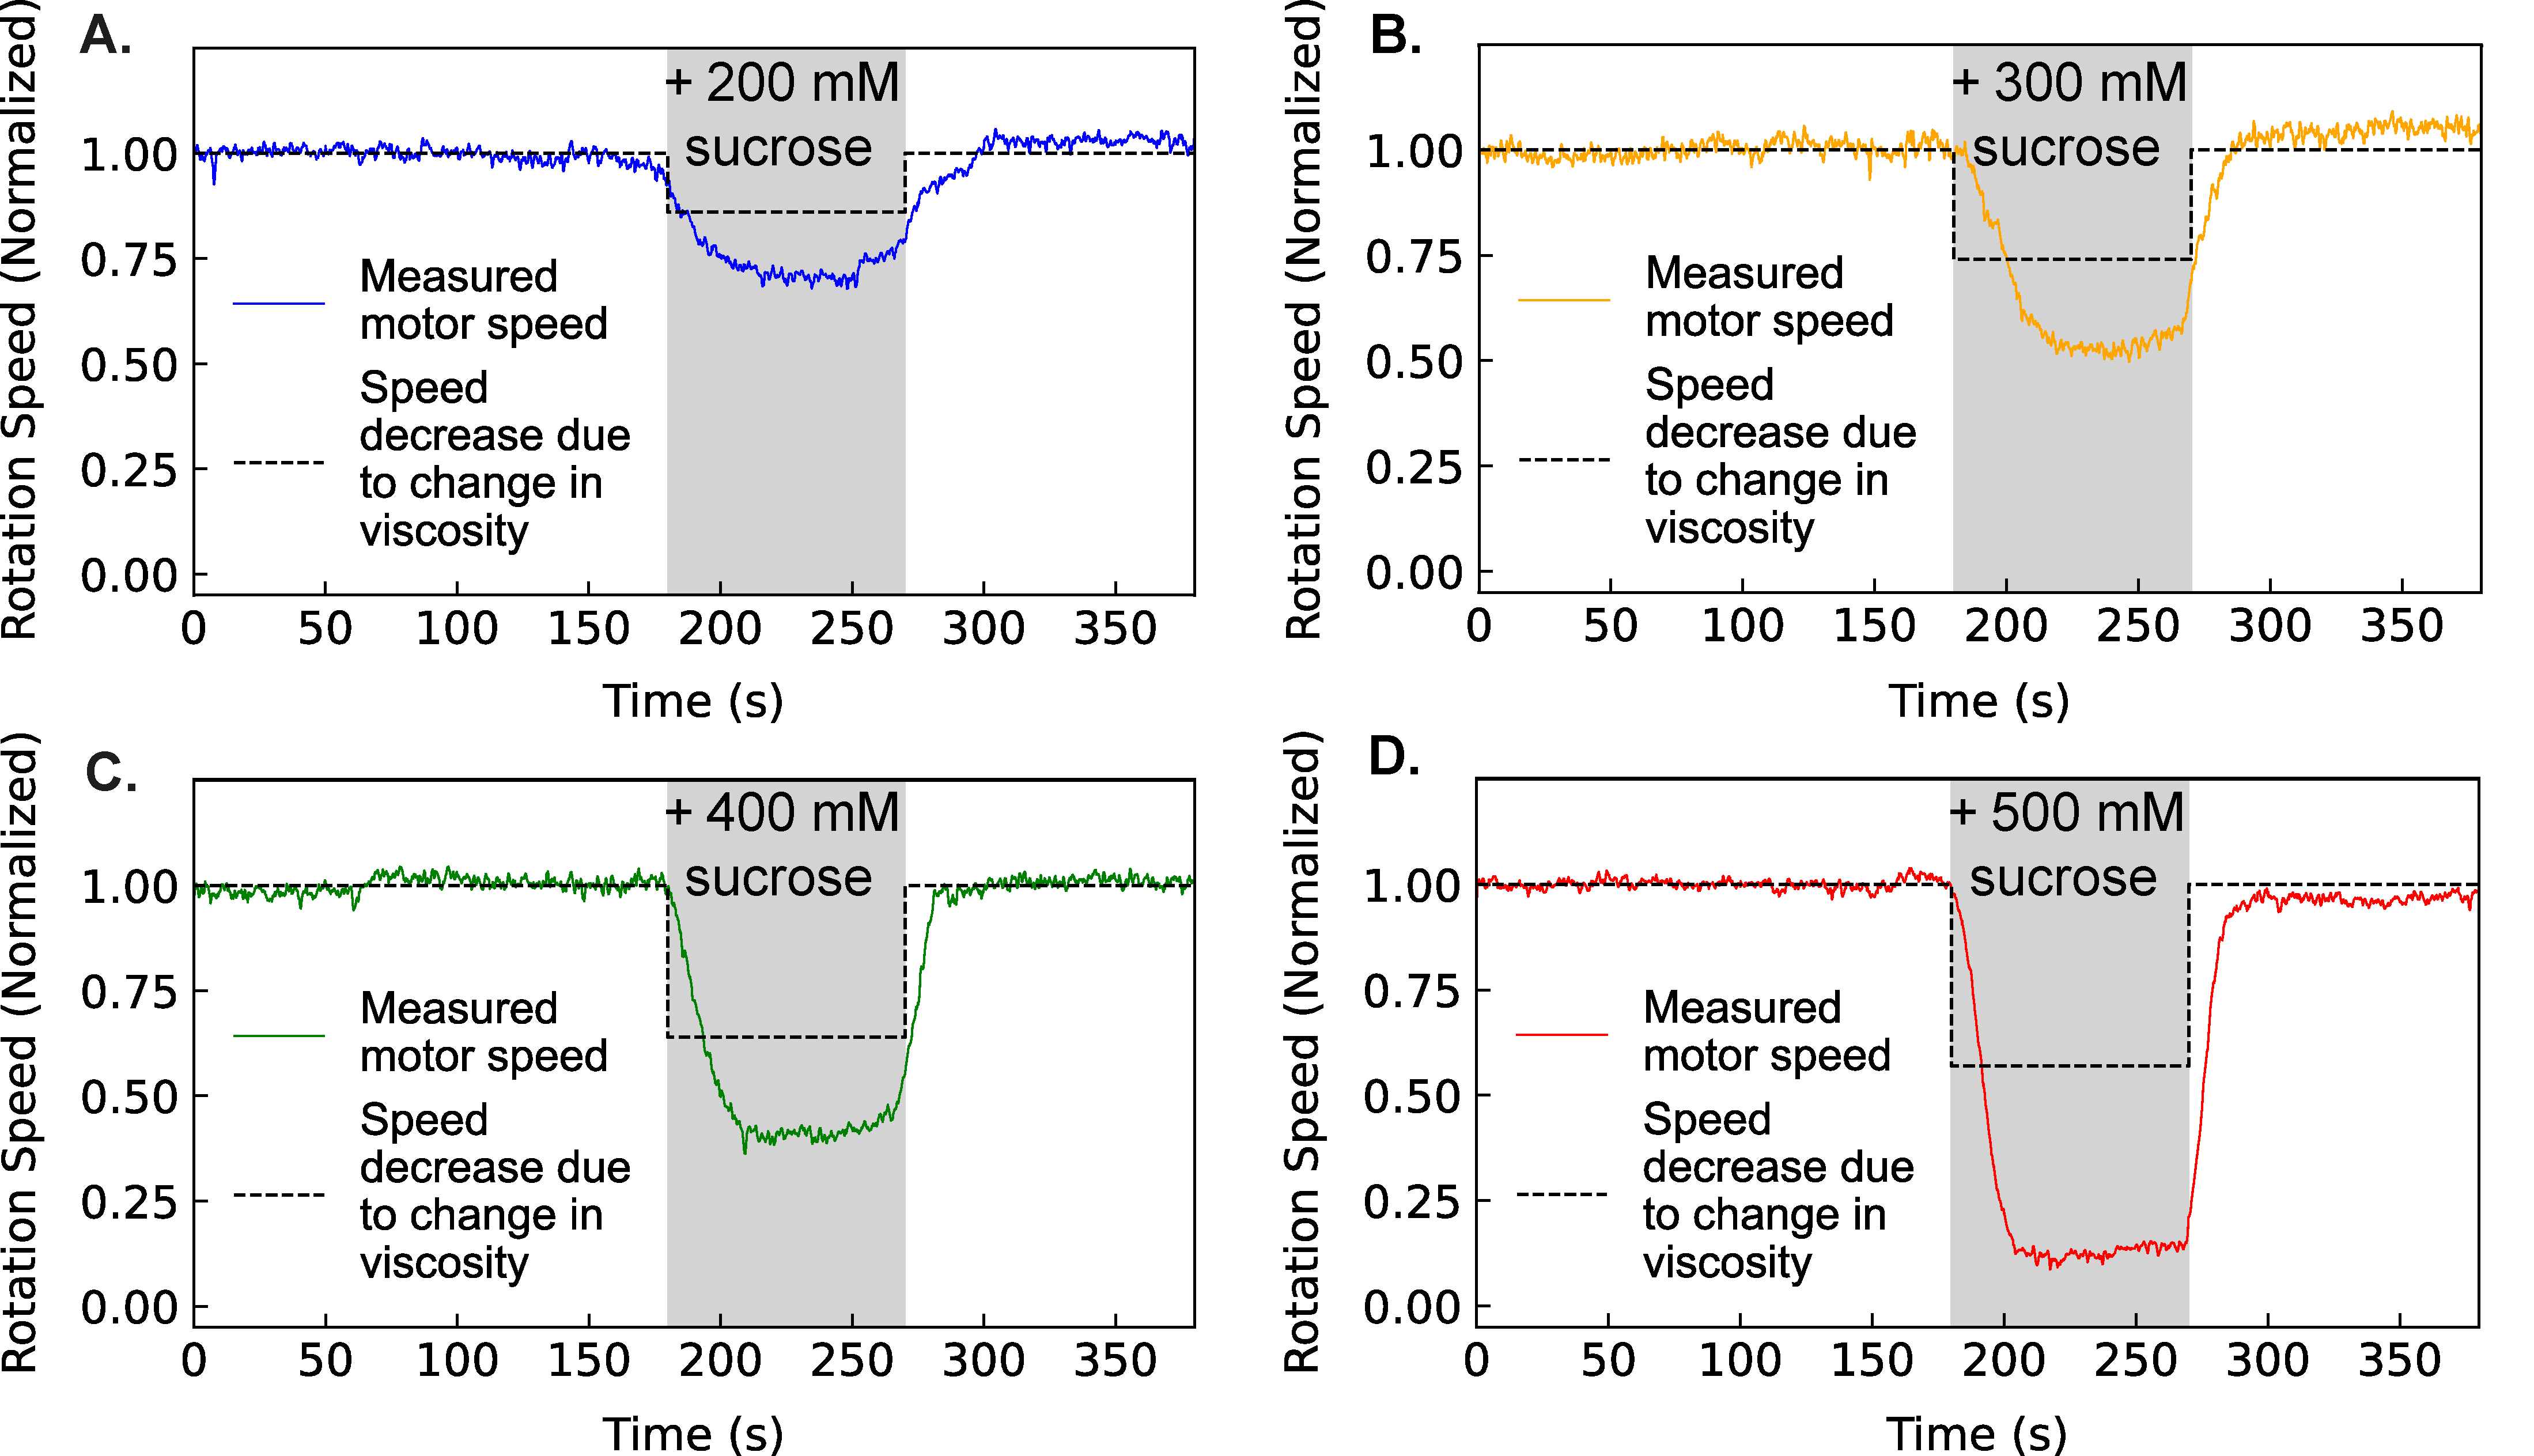
\includegraphics[width=\linewidth]{figures/Viscosity-sucrose.pdf}
    \caption{\textbf{\textbf{Motor speed reduction during osmotic shock exceeds that expected from increased viscosity alone.}} 
    \textbf{A–D)} Population-averaged normalized rotation speeds during 200, 300, 400, and 500 mM sucrose shocks ($n$ = 8, 10, 8, and 12, respectively). Shaded regions indicate the duration of hyperosmotic exposure.
    Dashed black lines show the estimated changes in speed due solely to increased viscosity, calculated using Stokes' law. Estimated normalized speed reductions for 200, 300, 400, and 500 mM sucrose are 0.18, 0.26, 0.36, and 0.43, respectively. Observed speed reductions exceed these values, indicating a contribution from PMF dissipation beyond viscosity effects.}
    \label{sfig:viscosity-sucrose}
\end{figure*}


\begin{figure*}[htbp!]
    \centering
    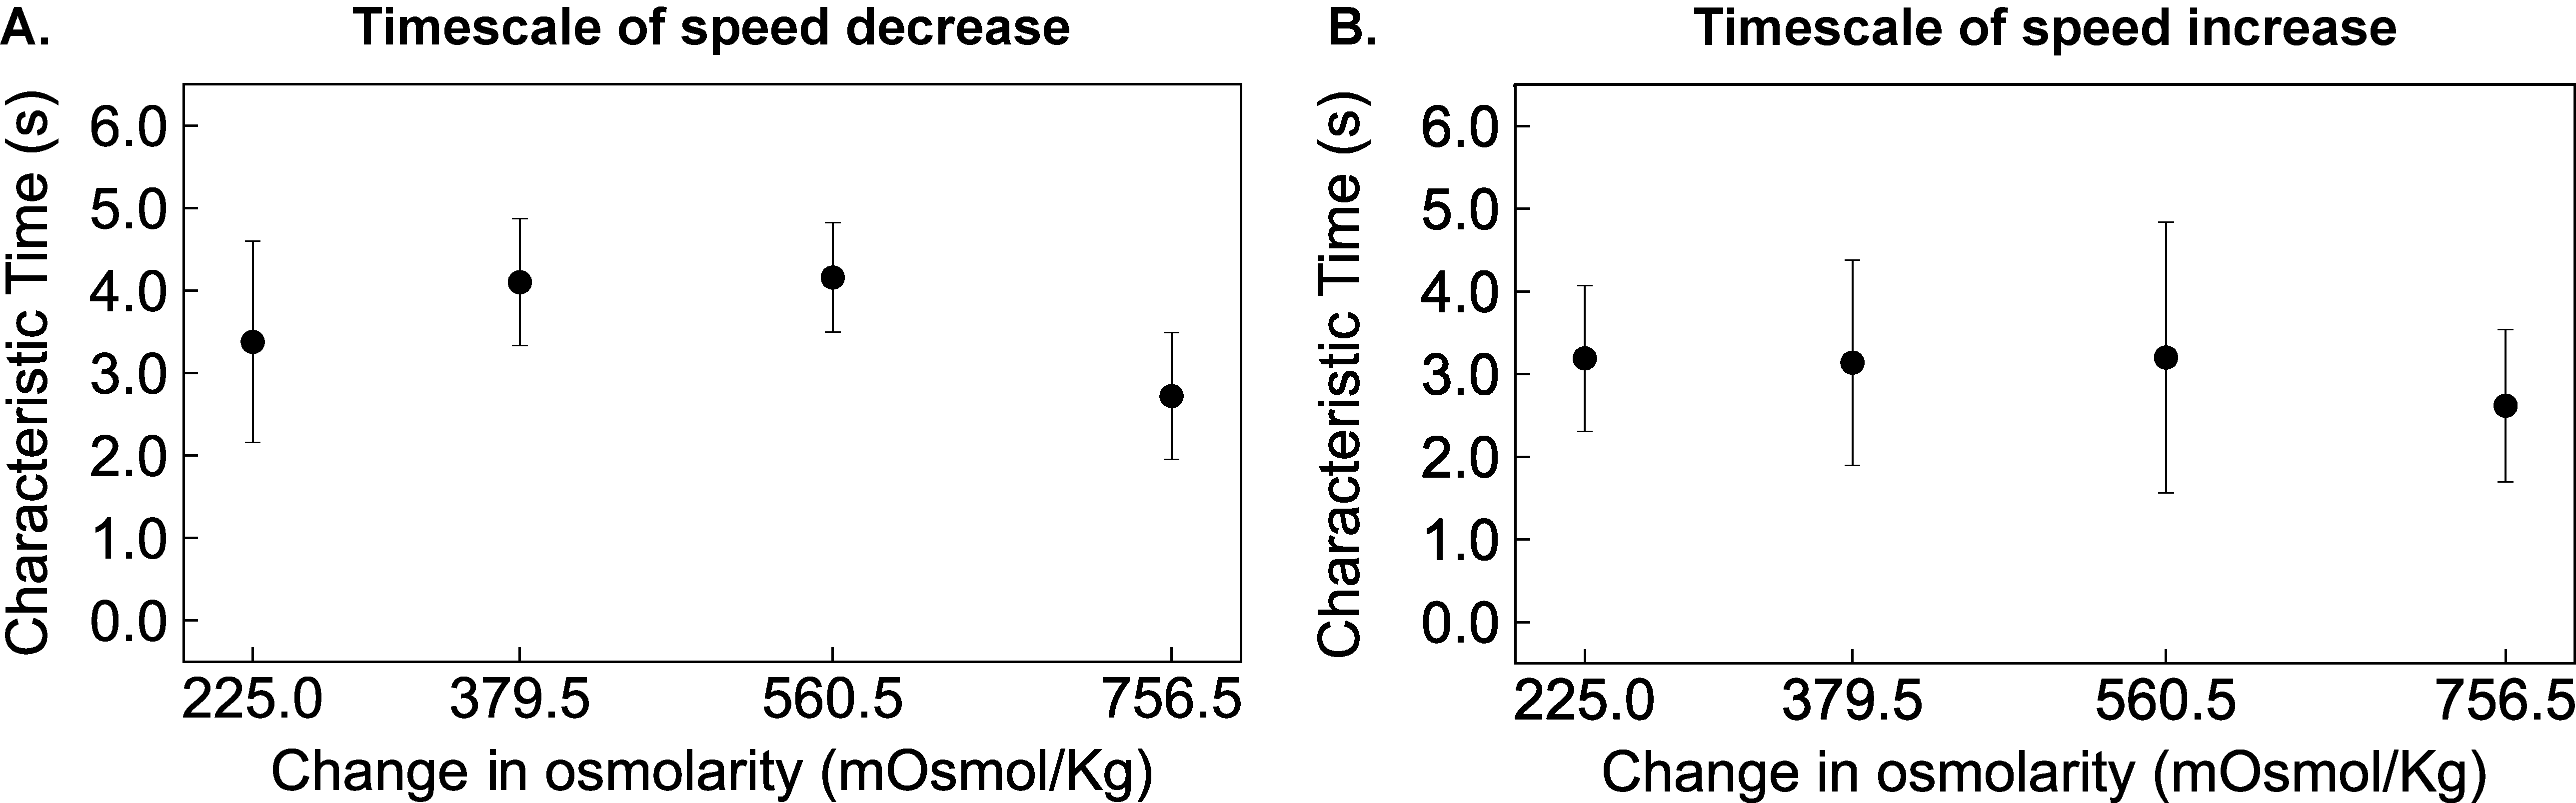
\includegraphics[width=\linewidth]{figures/sucros-time-charc.pdf}
   \caption{\textbf{Timescale of rotation speed as a function of change in osmolarity (from sucrose in MB)} \textbf{A)} Characteristic time for speed decrease during the decline phase, with black circles and error bars indicating mean and SD, respectively. \textbf{B)} Characteristic time for speed increase during the recovery phase, with black circles and error bars indicating mean and SD, respectively. Characteristic time shows no significant dependence on shock for either the decline or recovery phase.
}
    \label{sfig:tau-sucro-increa-decrease}
\end{figure*}




\begin{figure*}[htbp!]
    \centering
    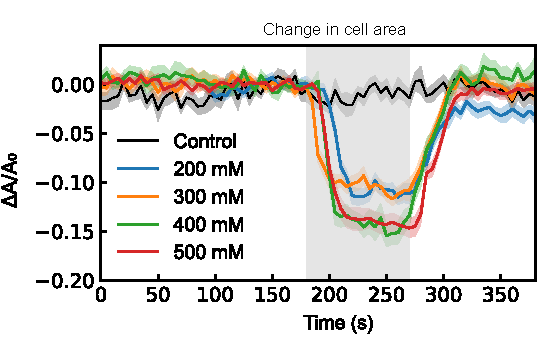
\includegraphics[width=0.6\linewidth]{figures/change-in-cell-area.pdf}
    \caption{\textbf{Cell area decreases transiently following hyperosmotic shock.} Population-averaged fractional change in cell area during 200--500~mM sucrose shocks and a 0~mM sucrose control ($n$ = 40 per condition). MG1655 cells were grown to OD$_{600}$= 0.5, washed, and resuspended in a 1:10 dilution prior to imaging. Cell area was normalized as $\Delta A/A_{0} = (A_{t} - A_{0})/A_{0}$, where $A_{t}$ is the cell area at time $t$ and $A_{0}$ is the mean pre-shock value. Cell area decreased during the shock in a dose-dependent manner and recovered upon return to base media. Shaded regions indicate the duration of hyperosmotic exposure. Solid lines and shaded bands represent mean and SE, respectively.}
    \label{sfig:cell-area}
\end{figure*}

\begin{figure*}
    \centering
    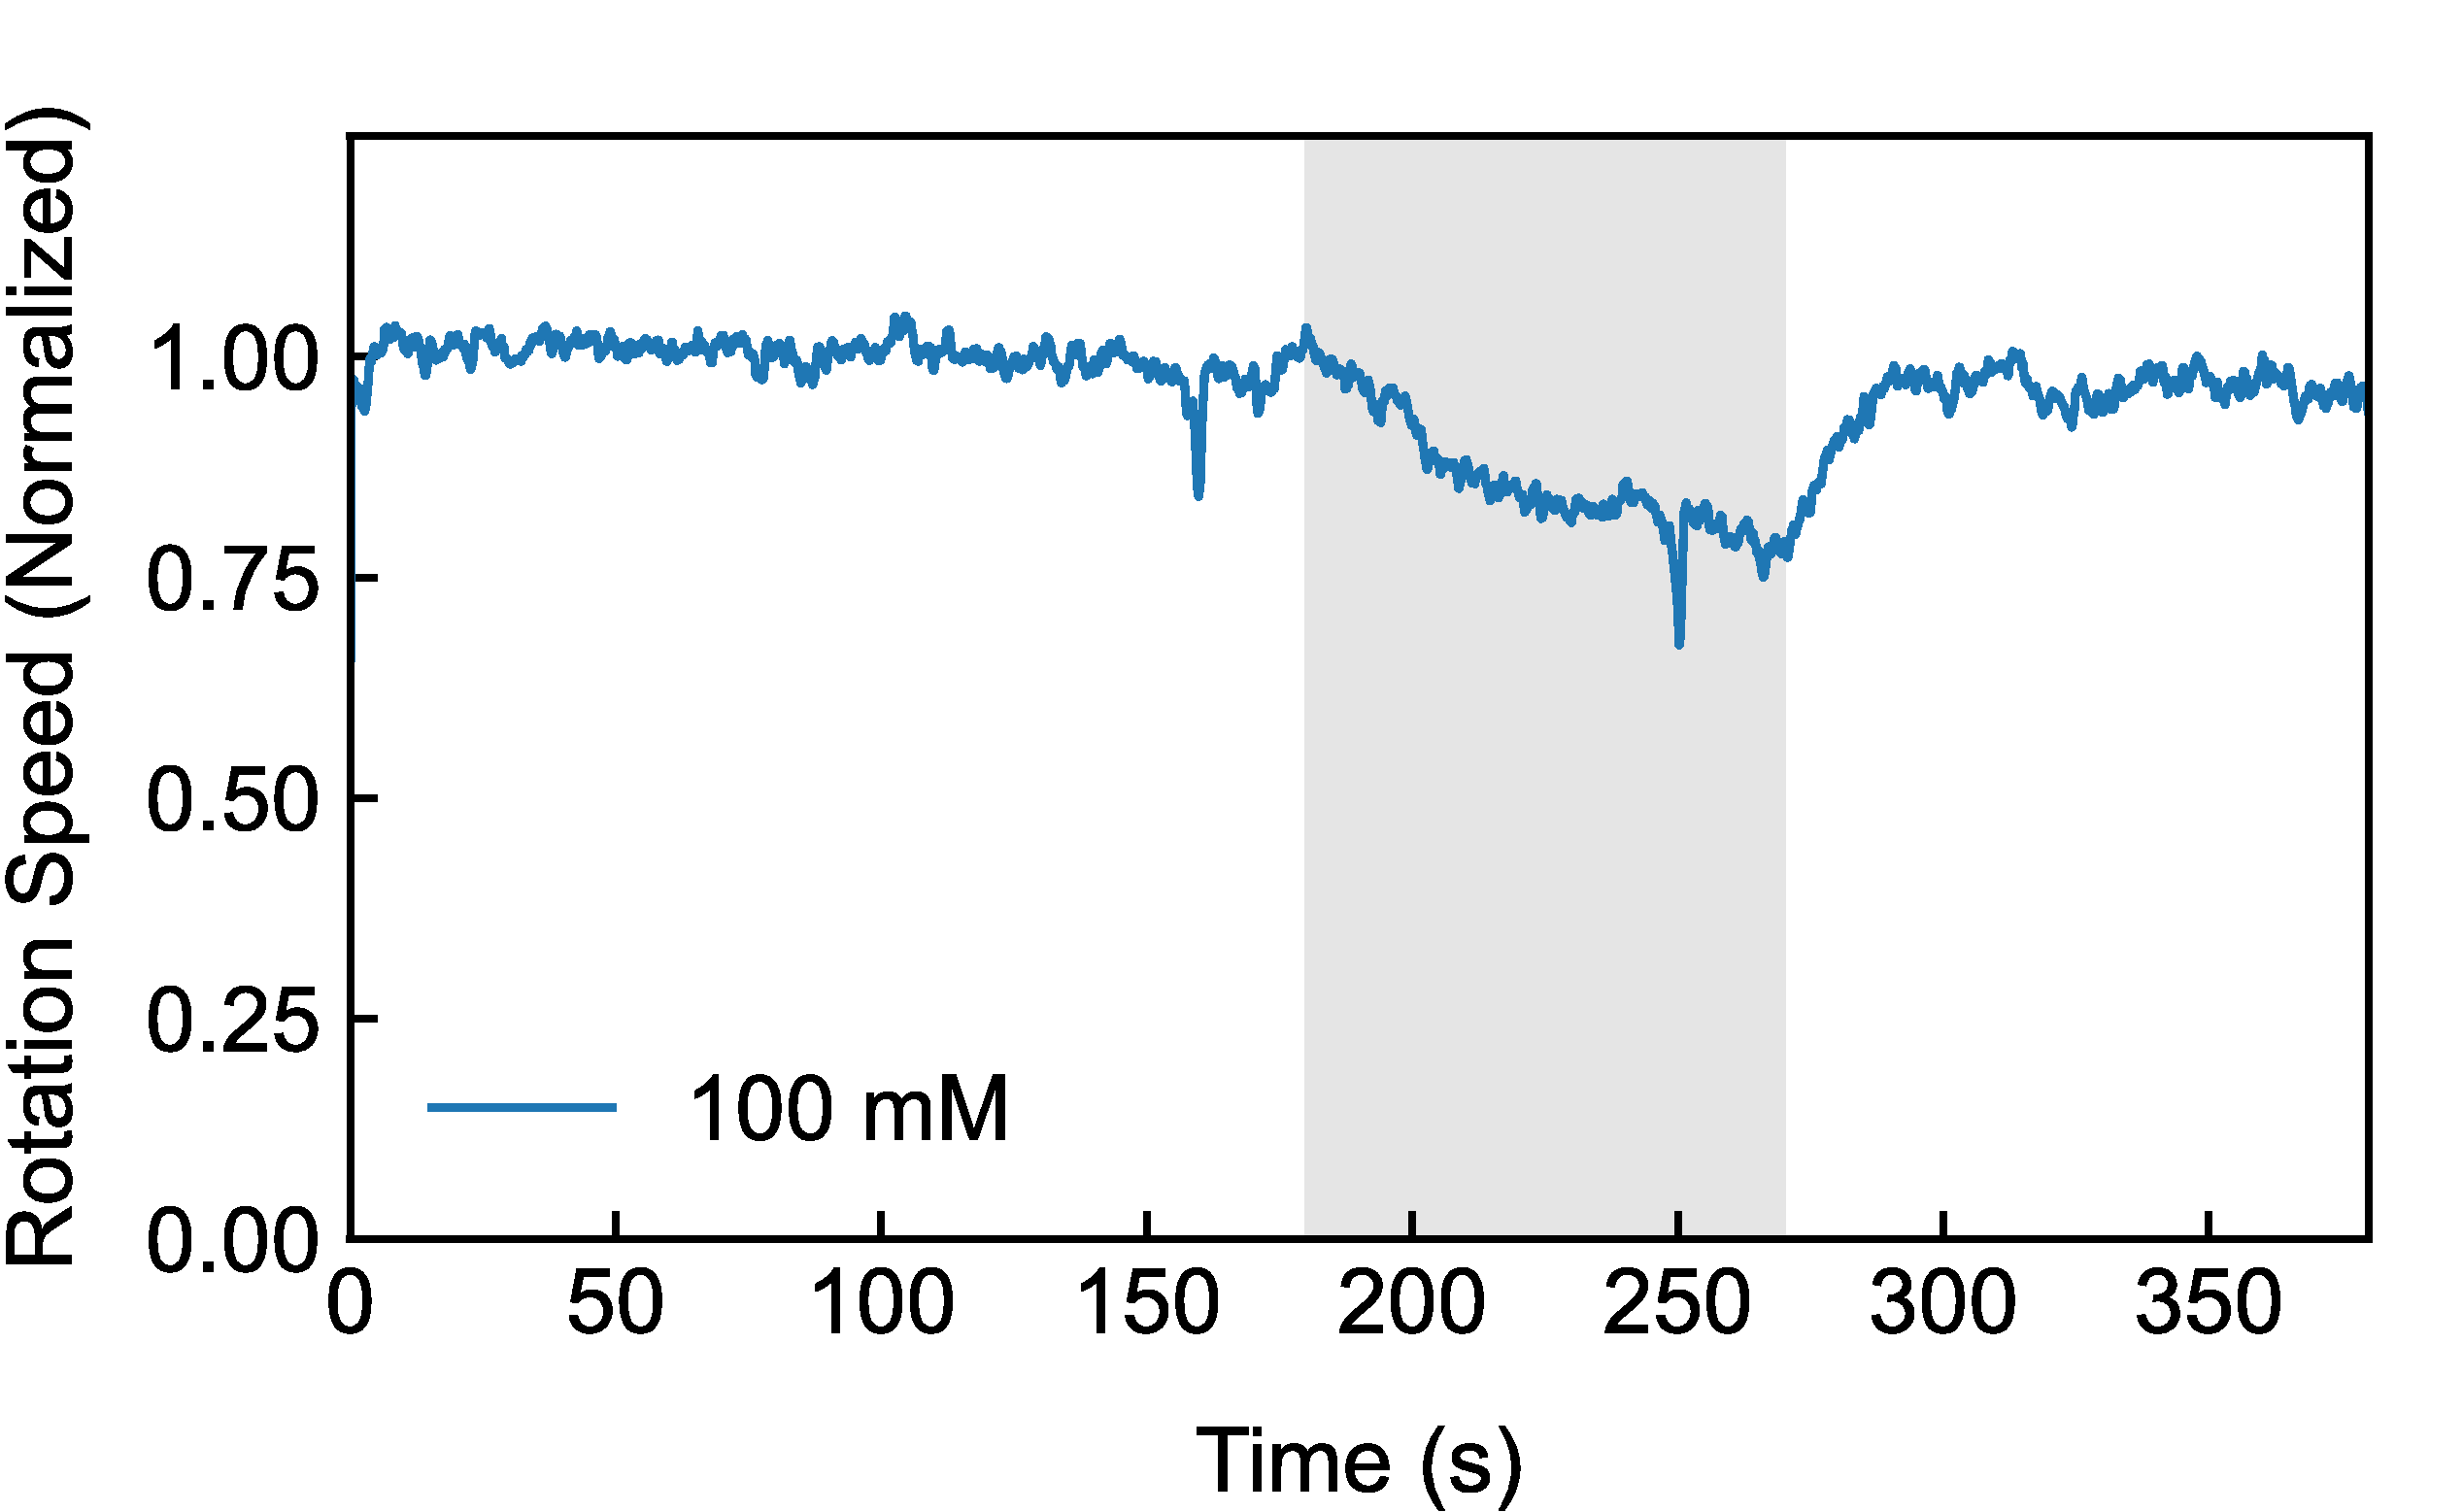
\includegraphics[width=0.6\linewidth]{figures/100mM.pdf}
    \caption{\textbf{Motor speed decrease during a 100~mM hyperosmotic shock.} Population-averaged normalized rotation speed during exposure to 100~mM sucrose shock ($n$ = 9). Motor speed decreased upon addition of sucrose and remained reduced throughout the shock period, recovering upon return to base media. The shaded region indicates the duration of hyperosmotic exposure.} 
    \label{sfig:100mM-sucrose}
\end{figure*}


\begin{figure*}[htbp!]
    \centering
    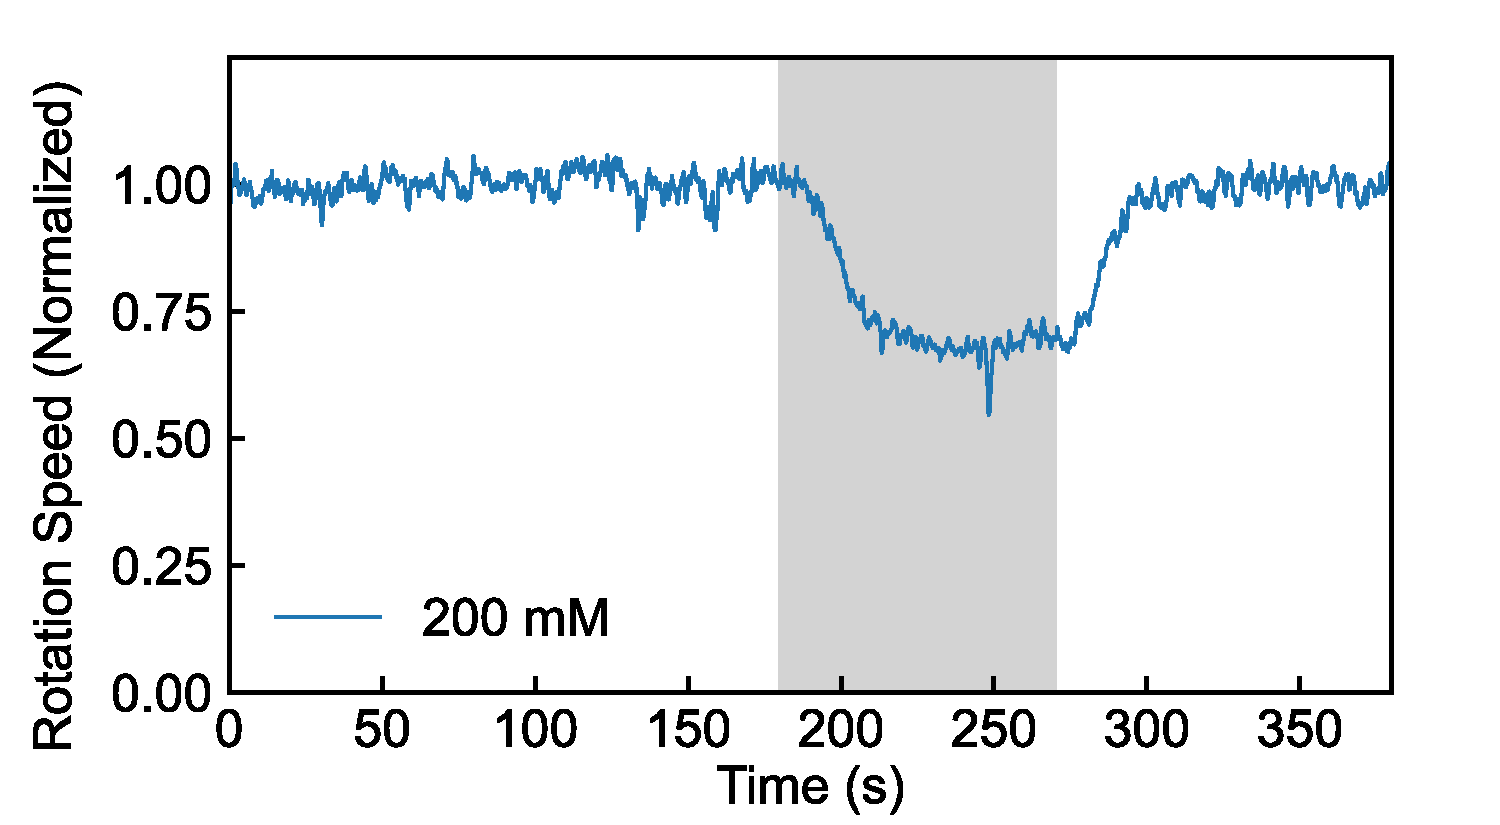
\includegraphics[width= 0.6\linewidth]{figures/200-osmopro-short.pdf} \caption{\textbf{Motor speed decreases during osmotic shock in the presence of osmoprotectants.} Population-averaged normalized rotation speed during exposure to 200~mM sucrose with osmoprotectants ($n$ = 9). Motor speed decreased upon addition of sucrose and did not recover during the shock period. The shaded region indicates the duration of hyperosmotic exposure.}
    \label{sfig:200_short_osmopro}
\end{figure*}





\begin{figure*}[htbp!]
    \centering
    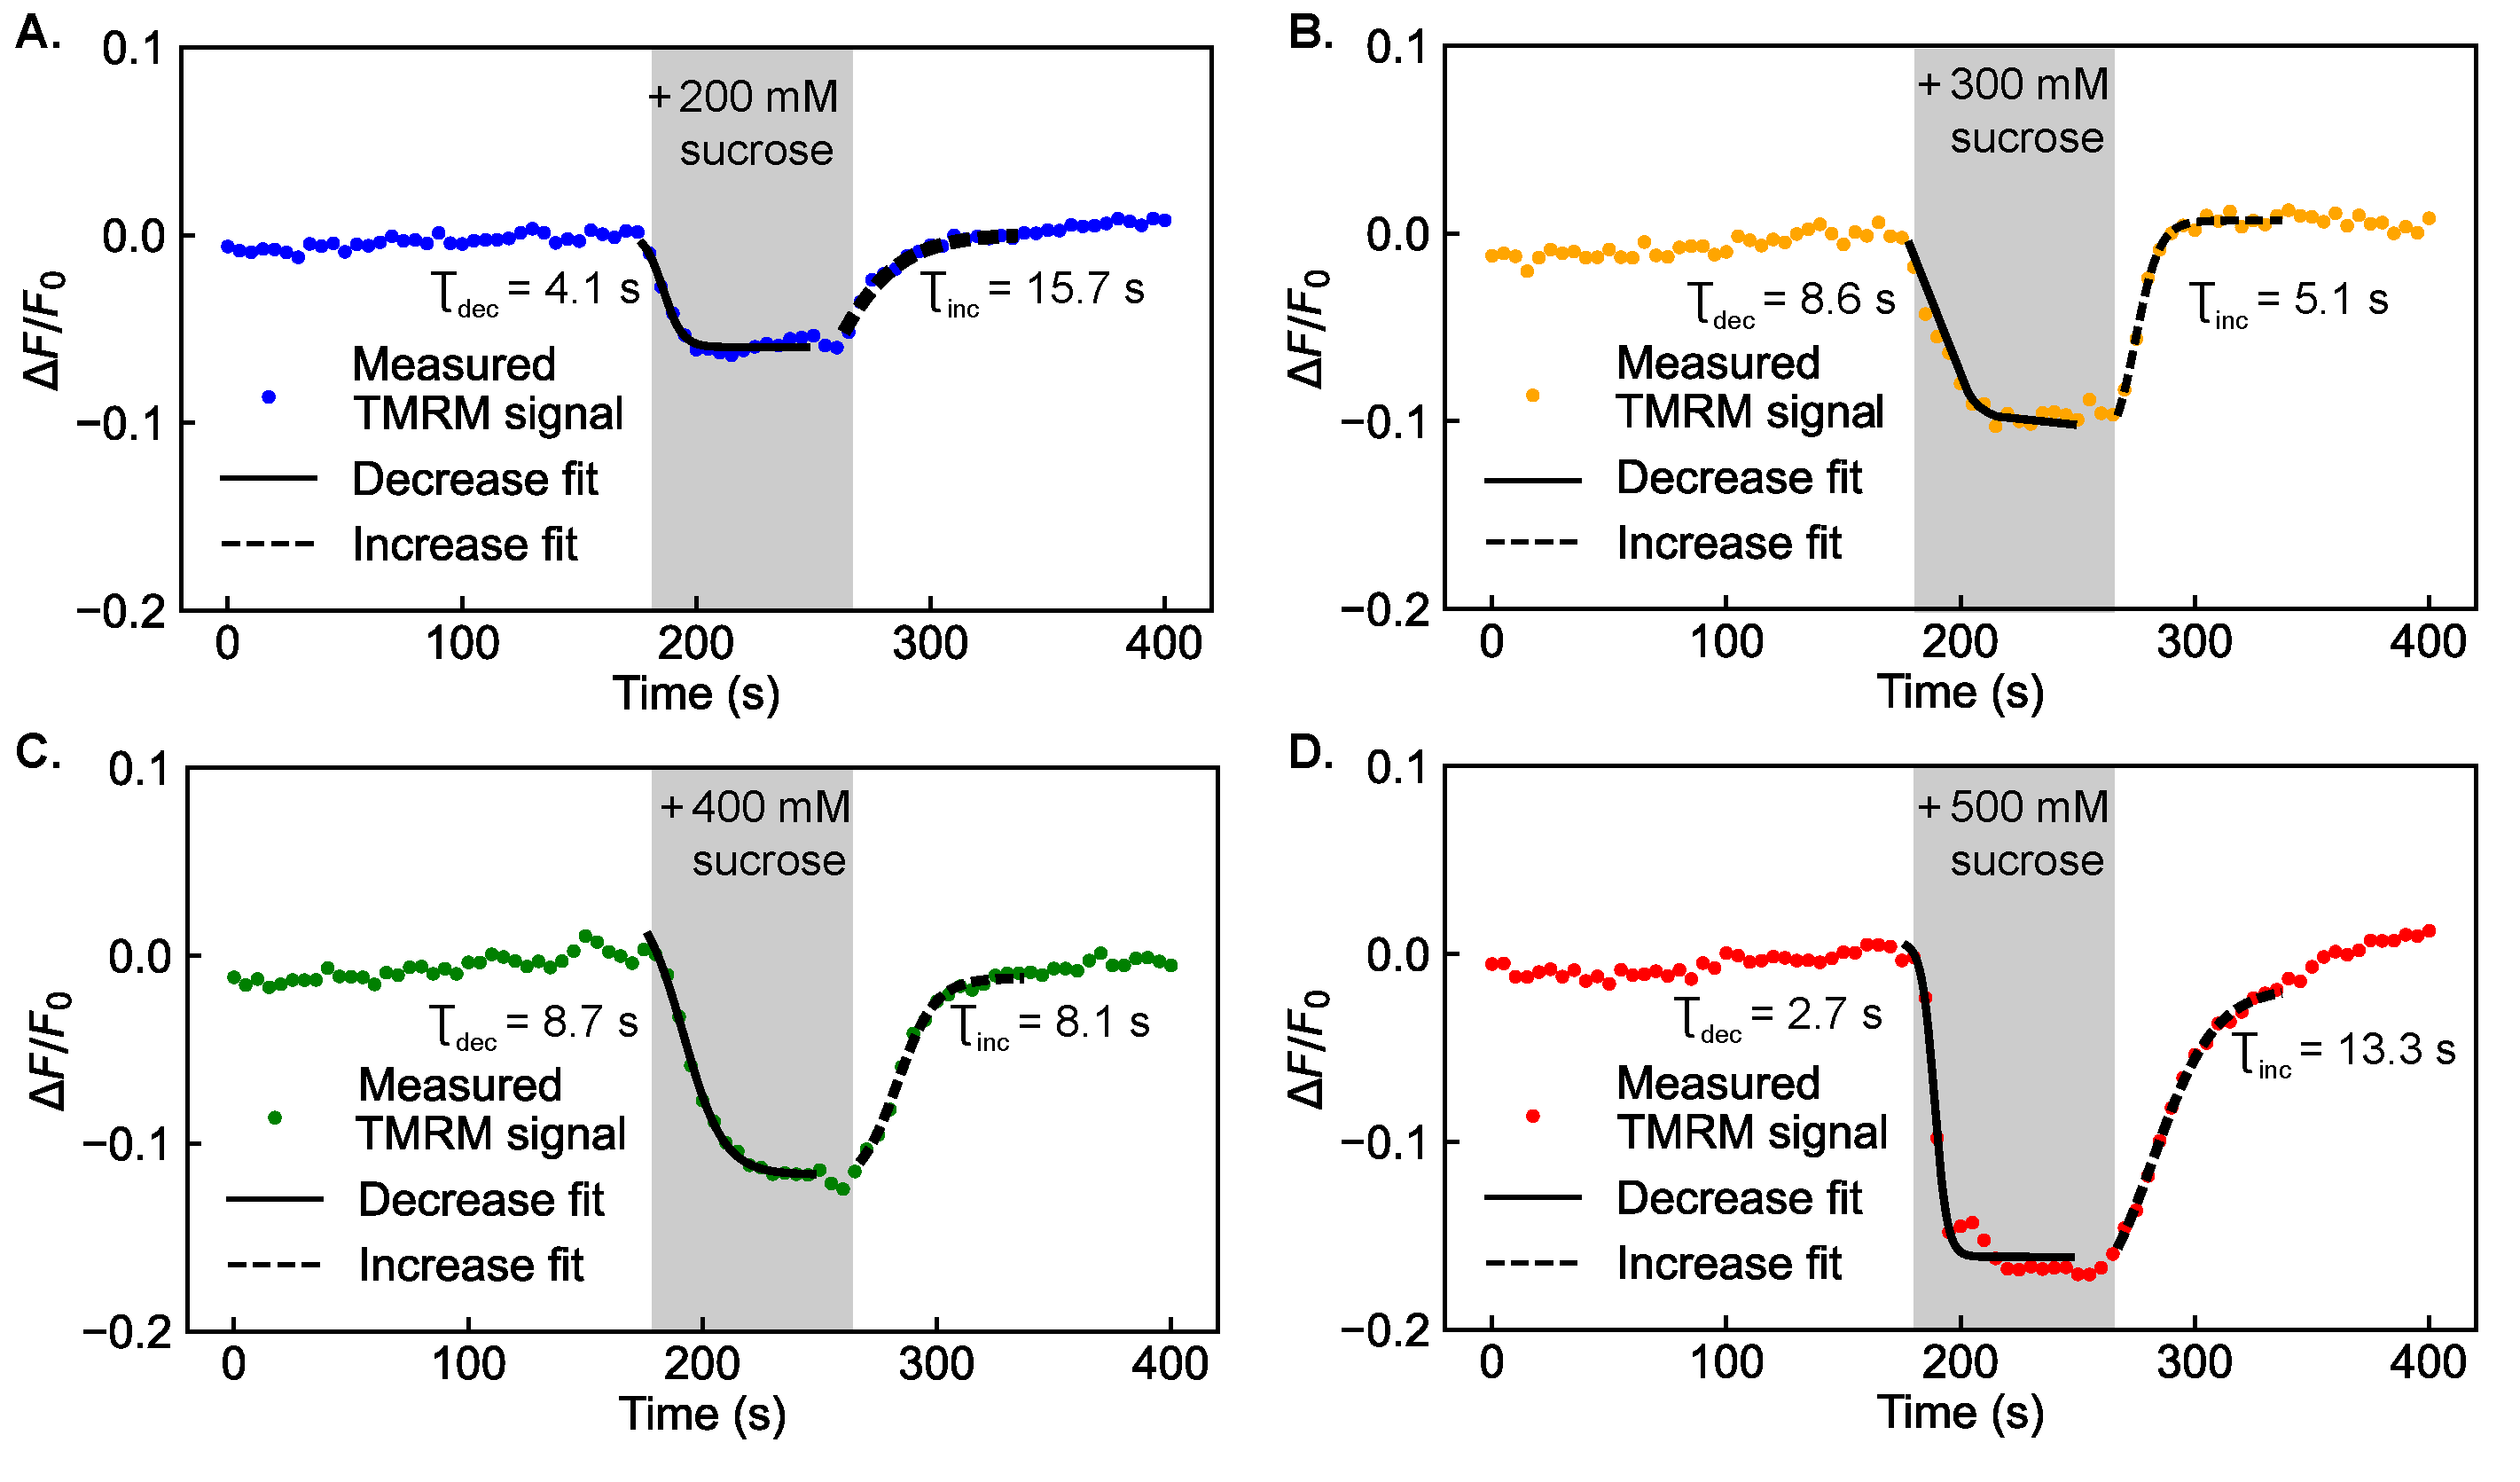
\includegraphics[width=\linewidth]{figures/TMRM-timescales.pdf}
     \caption{\textbf{Timescale of decay and recovery of the TMRM signal during osmotic upshifts.} Population-averaged normalized TMRM fluorescence during 200, 300, 400, and 500~mM sucrose-induced hyperosmotic shocks ($n$ = 40). Shaded regions indicate the duration of hyperosmotic exposure. A sigmoidal function,
    $ S(t) = S_0 - \frac{\Delta S}{1 + \exp\left(-\frac{t - t_0}{\tau}\right)}$, was used for curve fitting to quantify the characteristic timescales ($\tau$) of signal decrease and recovery, shown as solid and dashed lines, respectively.}
    \label{sfig:timescale-TMRM}
\end{figure*}




\newpage
\begin{figure*}[htbp!]
    \centering
    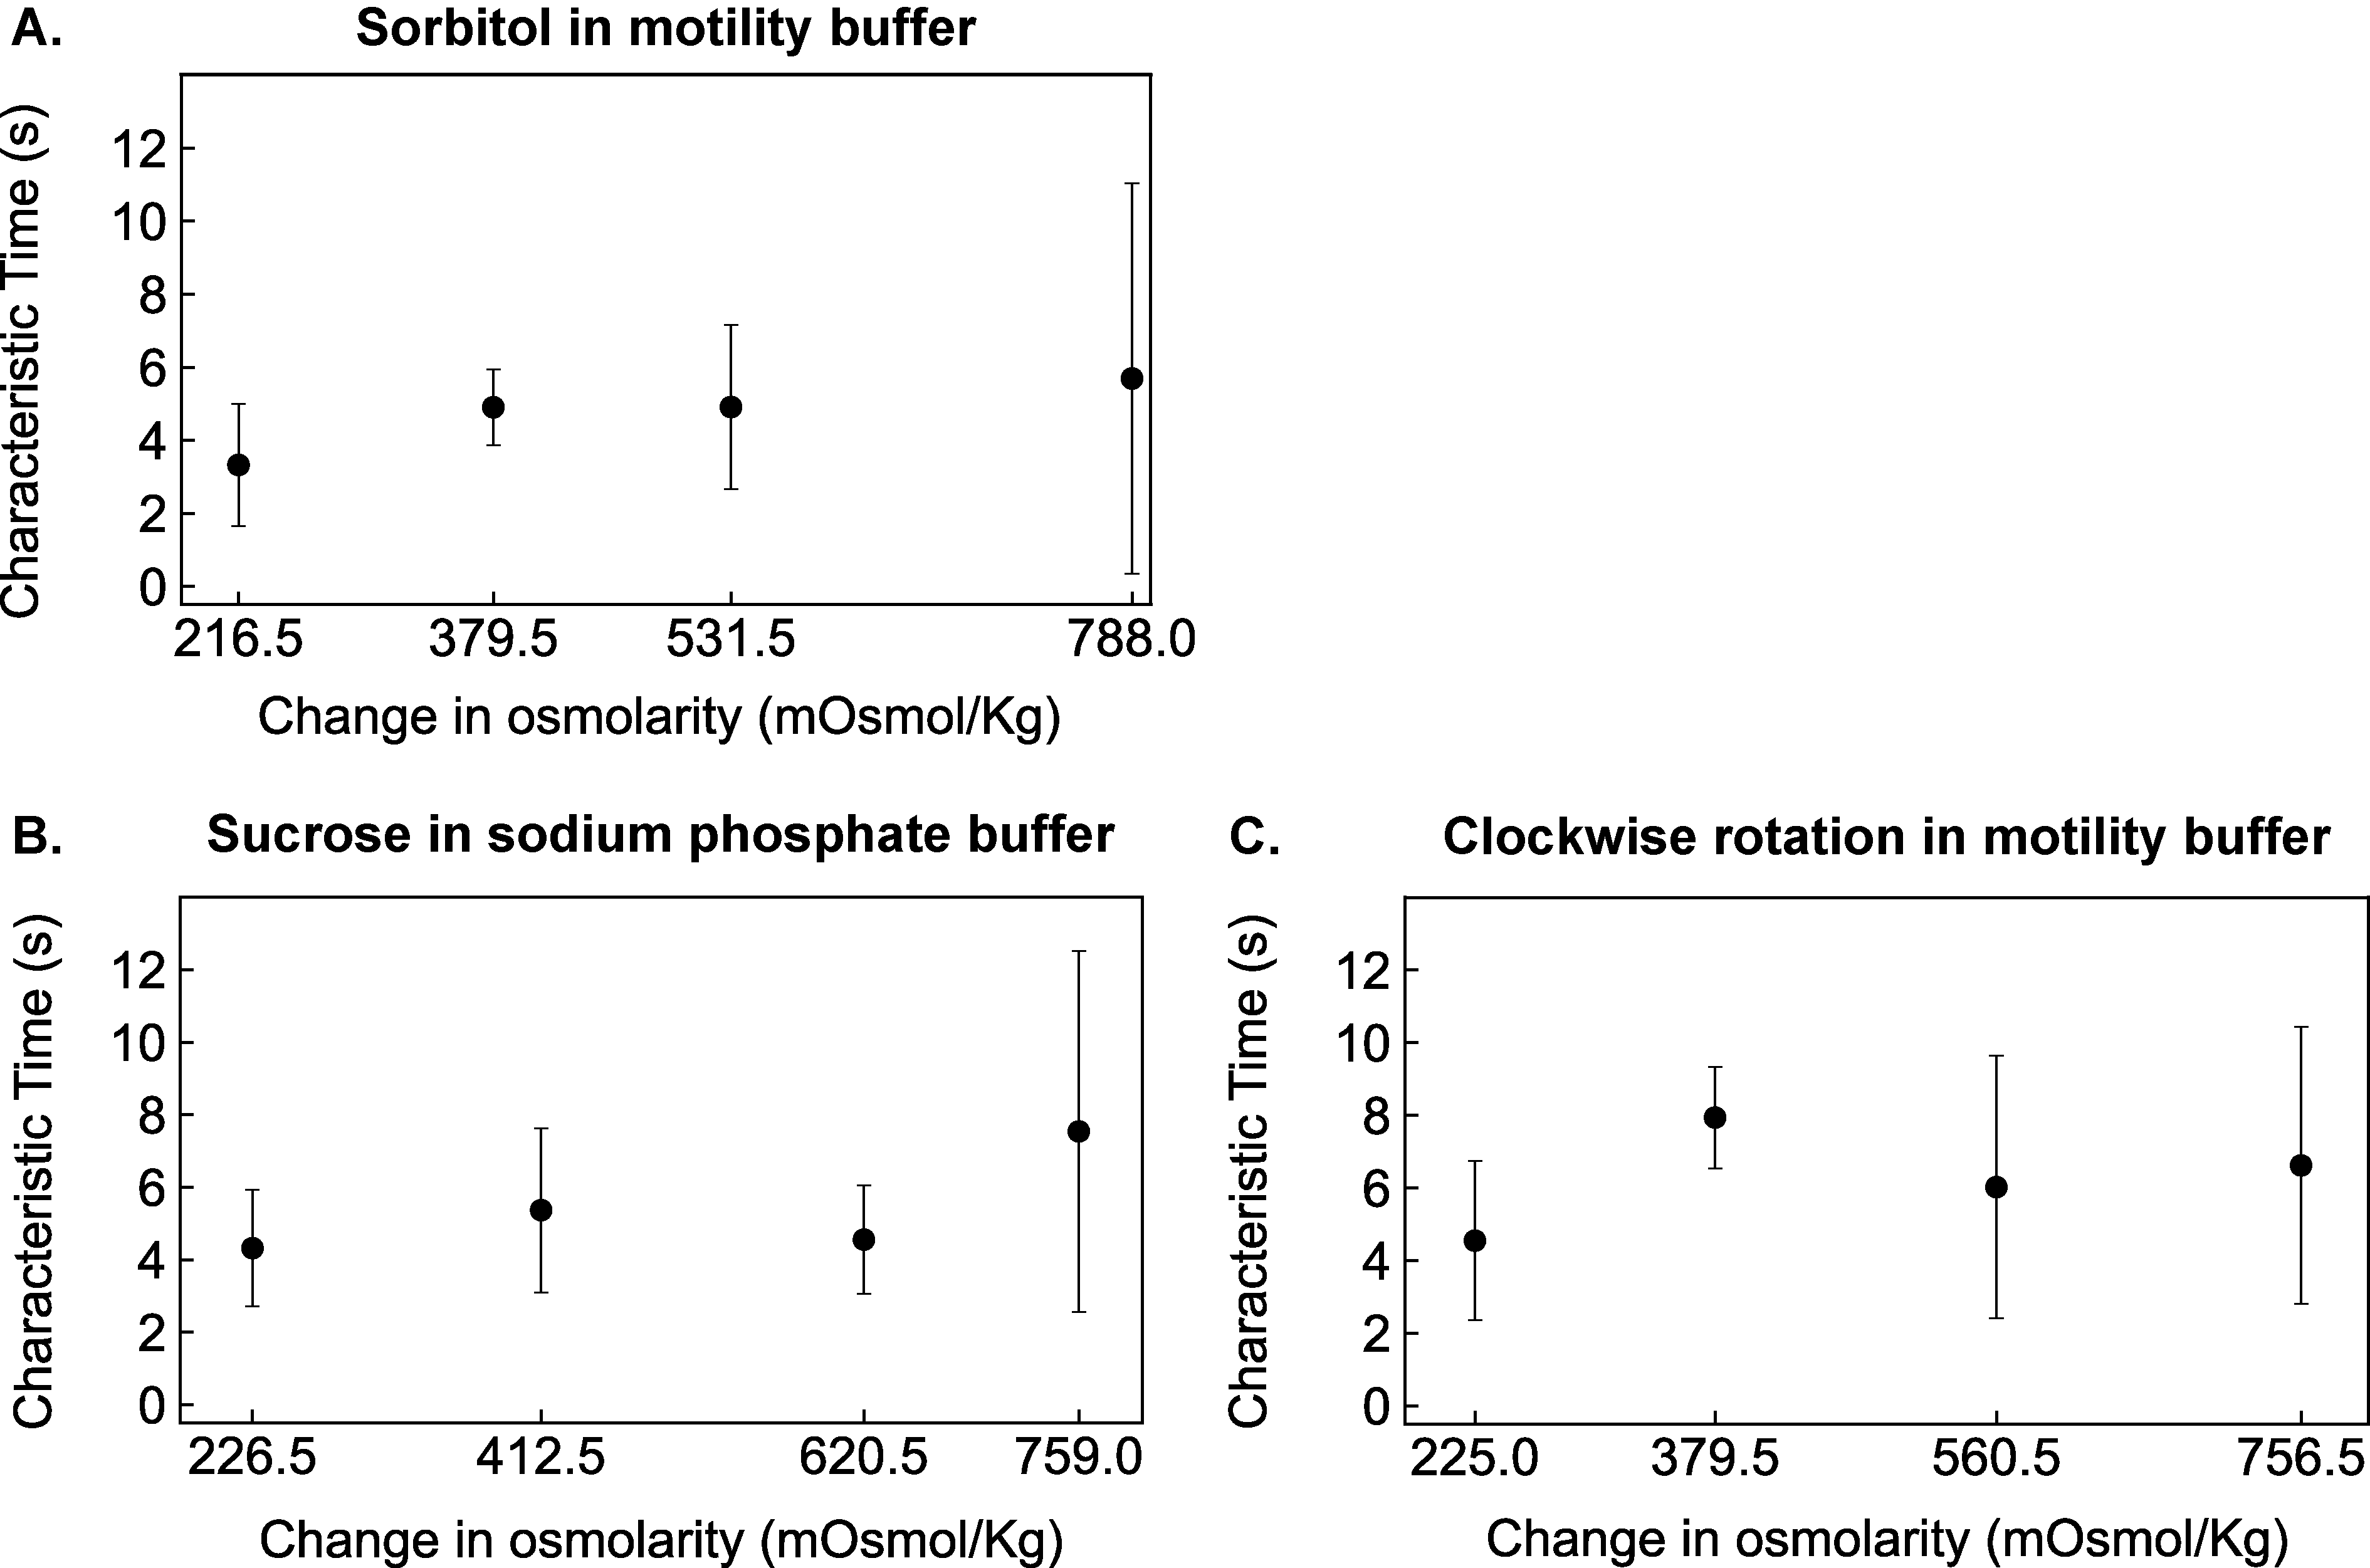
\includegraphics[width=\linewidth]{figures/Time-charact-sodium-sorb-clockwise.pdf}
   \caption{\textbf{Timescale of speed decrease as a function of change in osmolarity.} 
\textbf{A–C)} Characteristic time representing the timescale of speed decrease for: (\textbf{A}) sorbitol in MB, (\textbf{B}) sucrose in SPB, and (\textbf{C}) clockwise rotation of sucrose in MB. Black circles and error bars indicate the mean and SD, respectively. Characteristic time shows no significant dependence on shock strength.}
    \label{sfig:tau-sorb-sodium-clock}
\end{figure*}



\newpage
\begin{figure*}[htbp!]
    \centering
    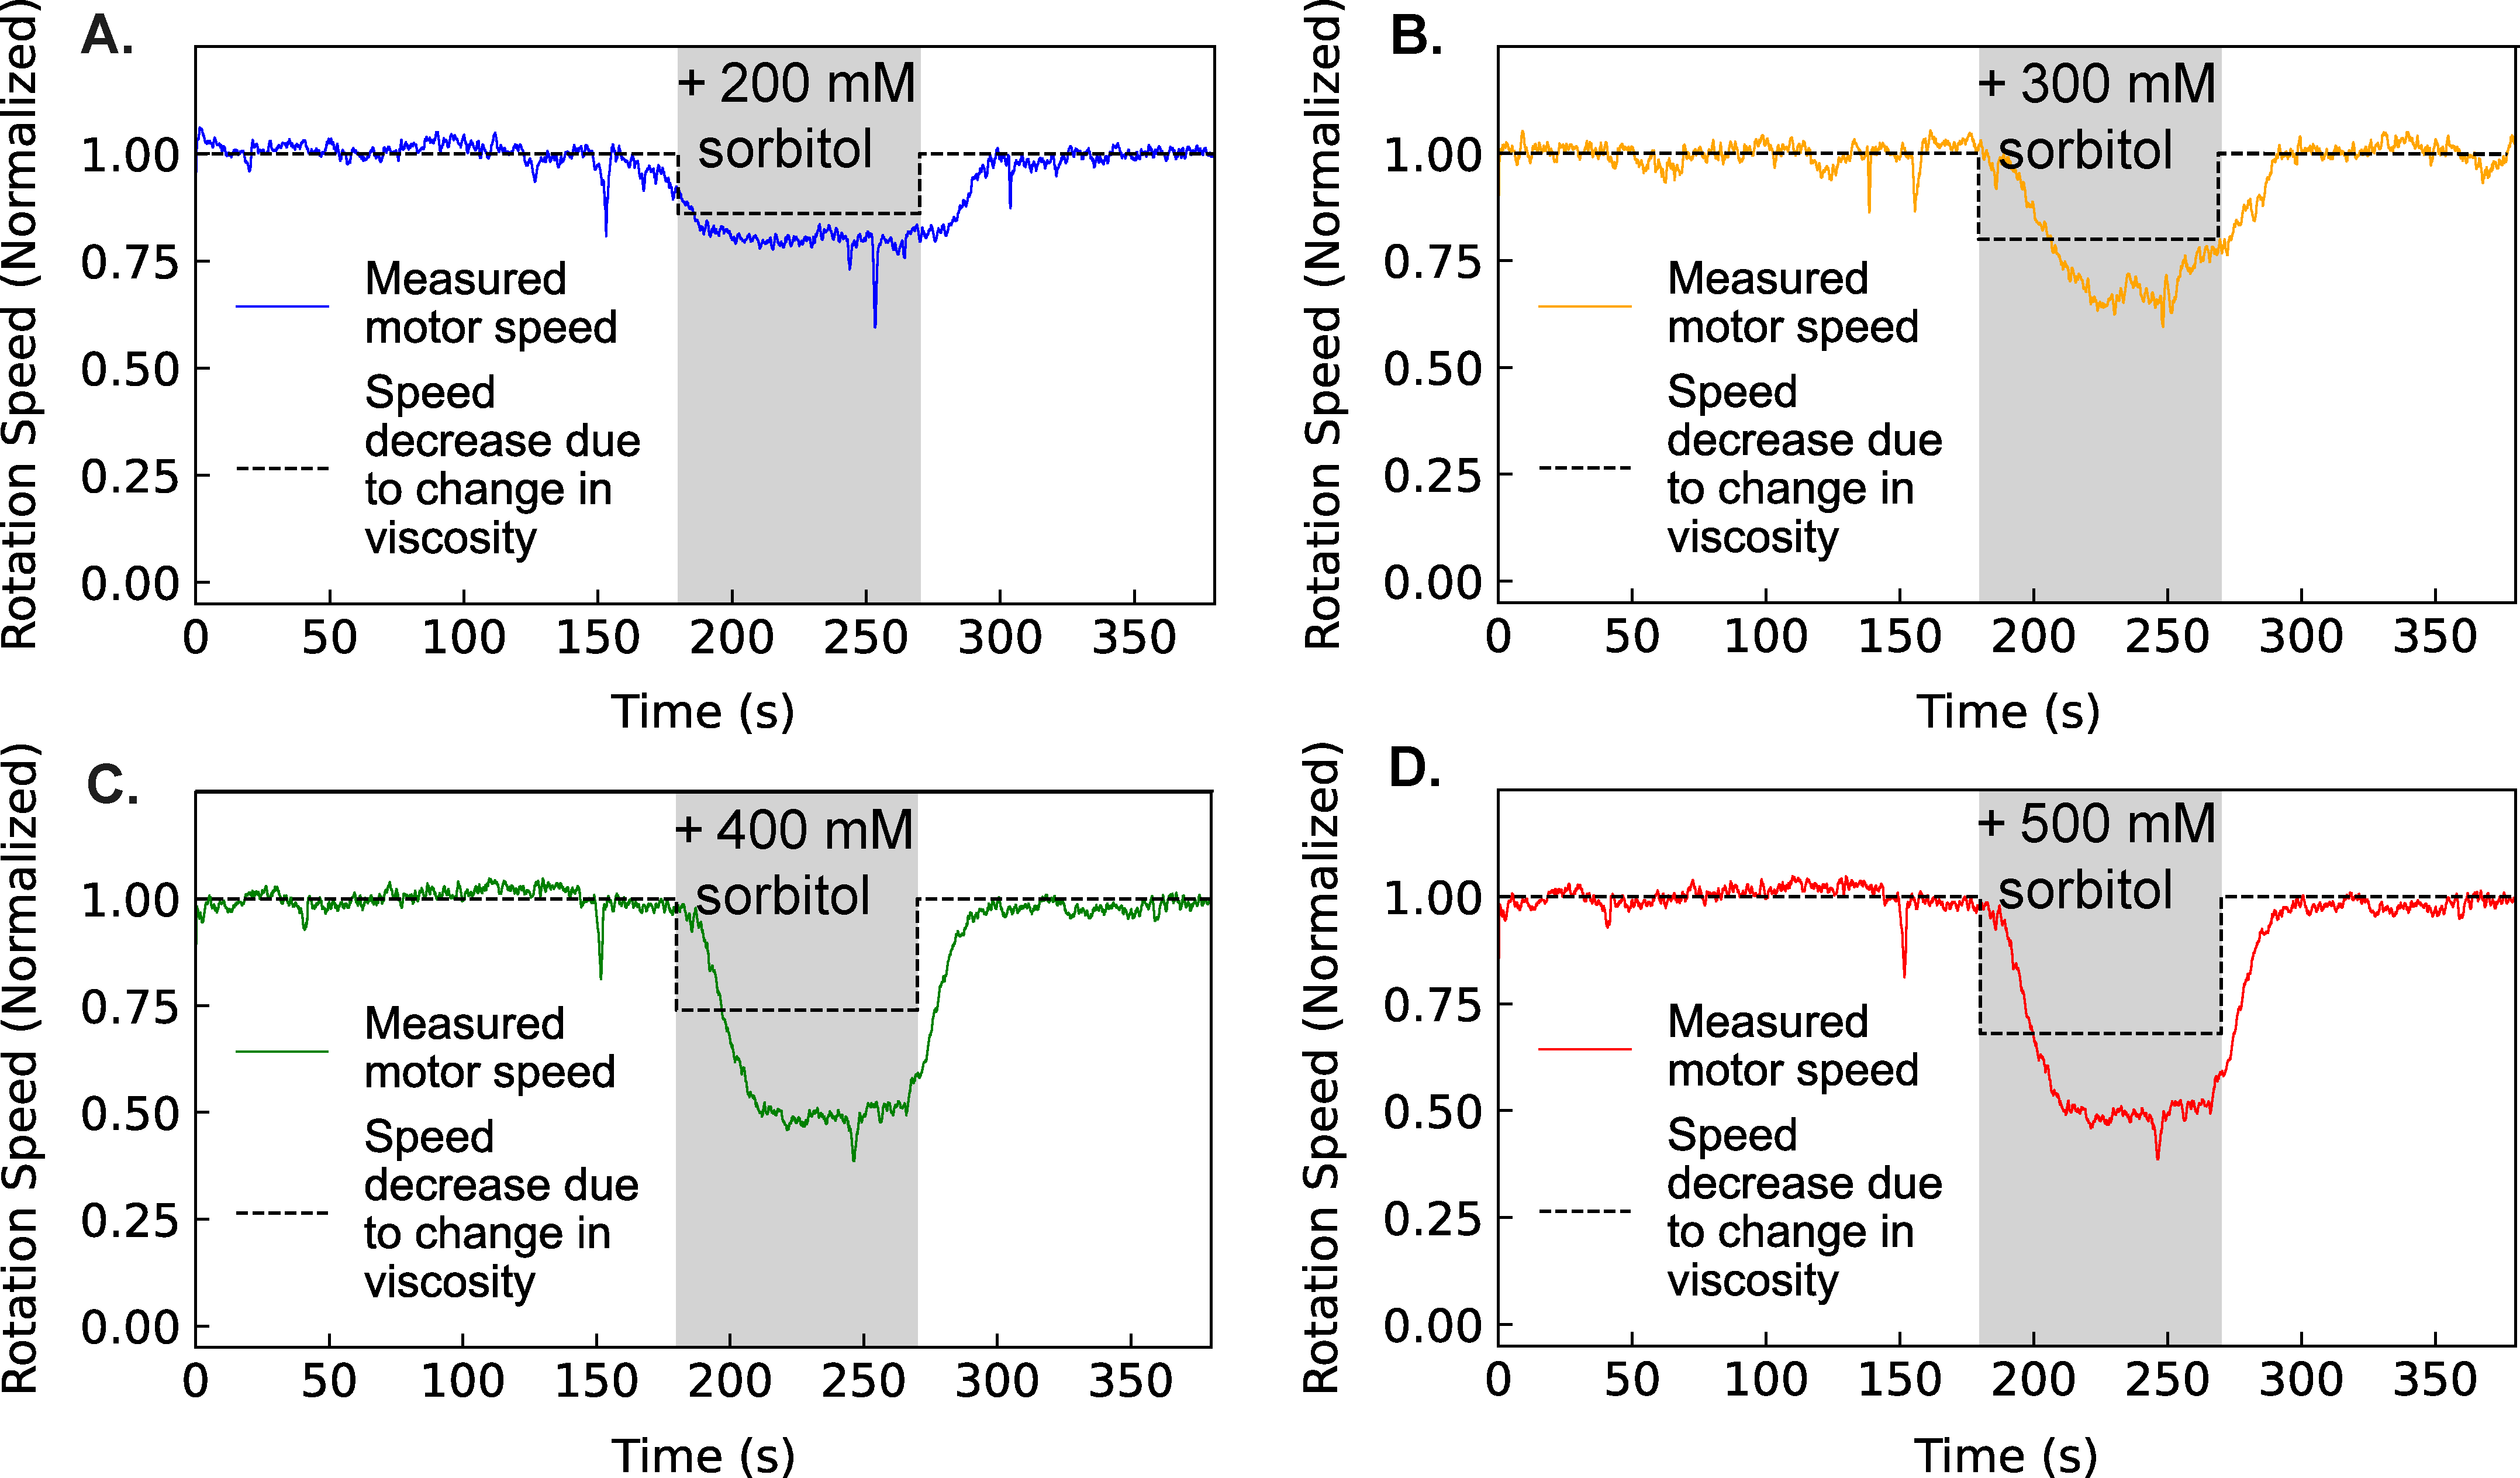
\includegraphics[width=\linewidth]{figures/Viscosity-Sorb.pdf}
    \caption{\textbf{\textbf{Motor speed reduction during osmotic shock exceeds that expected from increased viscosity alone.}} 
    \textbf{A–D)} Population-averaged normalized rotation speeds during 200, 300, 400, and 500 mM sorbitol shocks ($n$ = 8). Shaded regions indicate the duration of hyperosmotic exposure.
    Dashed black lines show the estimated changes in speed due solely to increased viscosity, calculated using Stokes' law. Estimated normalized speed reductions for 200, 300, 400, and 500 mM sorbitol are 0.14, 0.20, 0.26, and 0.32, respectively. Observed speed reductions exceed these values, indicating a contribution from PMF dissipation beyond viscosity effects.}
    \label{sfig:viscosity-plot-Sorb}
\end{figure*}




\newpage
\begin{figure*}[htbp!]
    \centering
    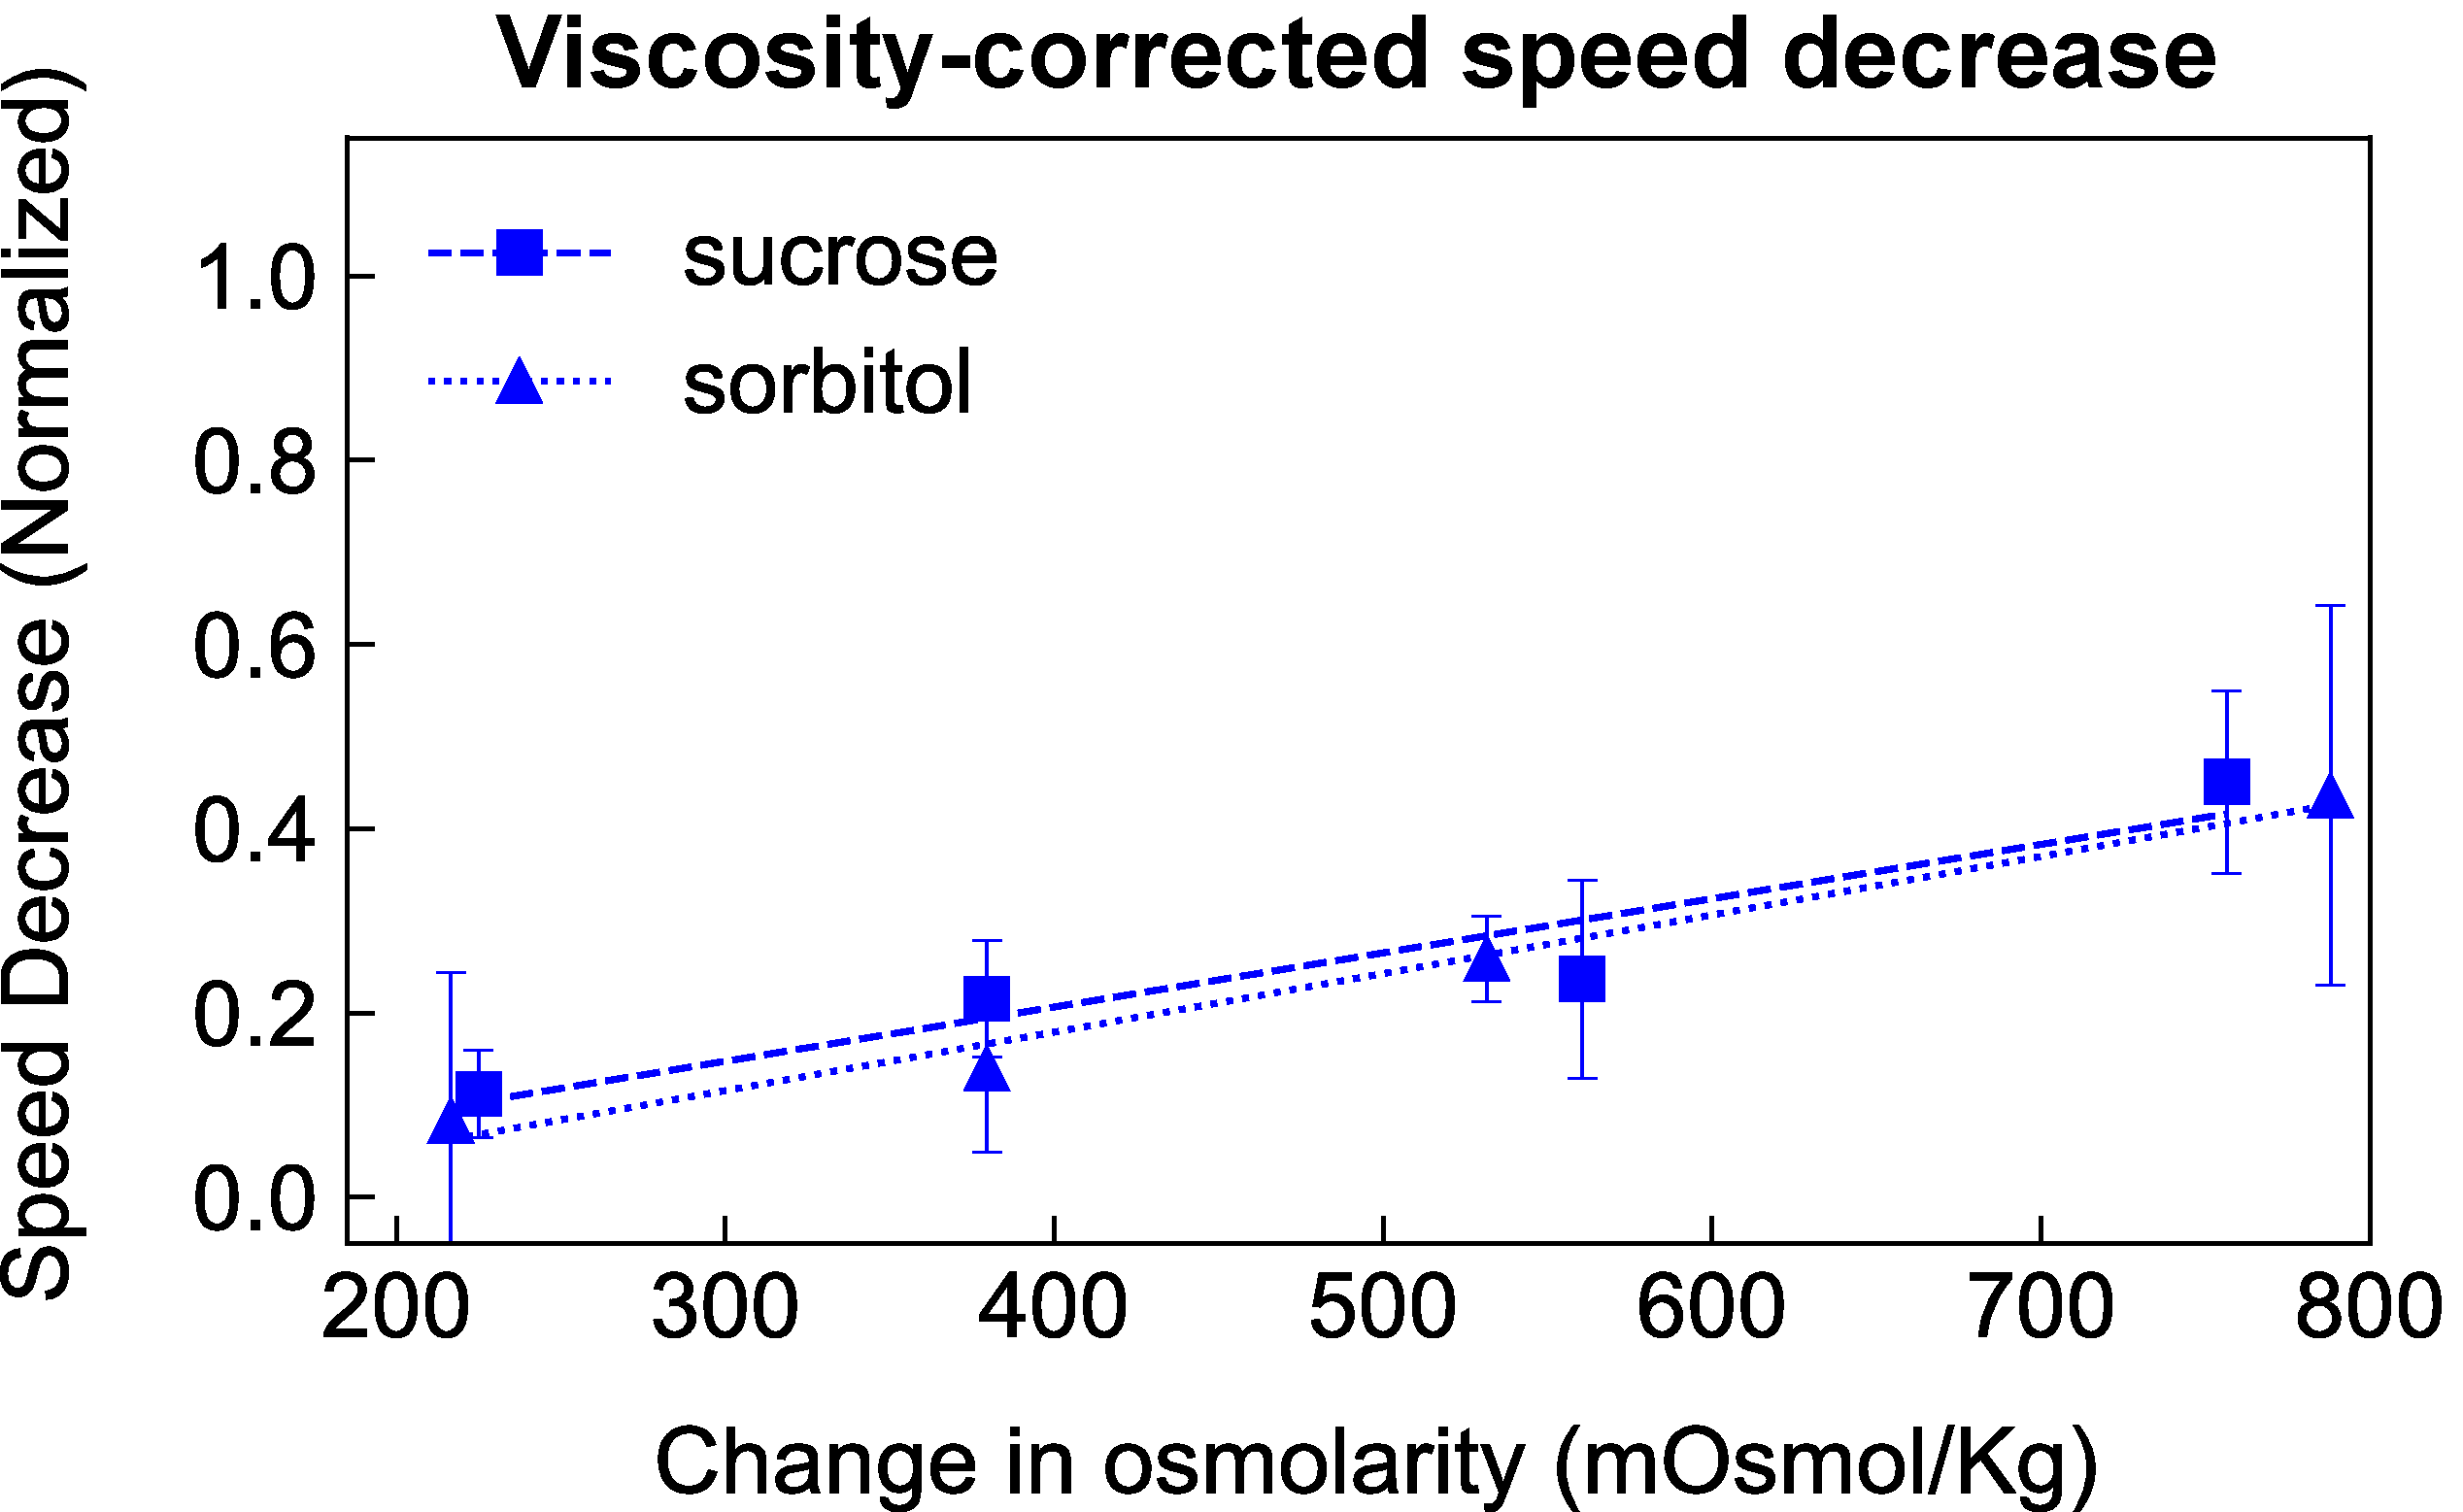
\includegraphics[width= 0.6\linewidth]{figures/sucrose-sorb-combin-speed-decrease.pdf} \caption{\textbf{Normalized speed reduction versus change in osmolarity for sucrose (dashed line) and sorbitol (dotted line).} Blue markers and error bars represent the difference between the total speed decrease and the estimated reduction due to changes in viscosity. The dashed and dotted lines show linear fits to this difference. Statistical values for the linear fits are provided in (Table~\textit{\ref{tab:fit_all_conditions}}).}
    \label{sfig:tau-sorb-sucrose-combine}
\end{figure*}





%%%%%%%%%%%%%%%% SUPPLEMENTARY TABLES %%%%%%%%%%%%%%%

\clearpage
\begin{table*}
\centering
\caption{\textbf{Linear fit parameters for the estimated speed decrease due to changes in viscosity of sucrose and sorbitol solutions.}}
\label{tab:fit_only_viscosity}
\begin{tabular}{l S[table-format=1.1] S[table-format=1.3] S[table-format=1.2]}
\toprule
Condition & {$m \; (\times 10^{-4})$} & {$b$} & {$R^{2}$} \\
\midrule
Sucrose   & 4.7 & 0.078 & 0.99 \\
Sorbitol  & 3.1 & 0.079 & 0.98 \\
\bottomrule
\end{tabular}

\end{table*}
\begin{table*}
\centering
\caption{\textbf{Linear fit parameters for each experimental condition.} The total speed decrease was determined from the mean and SD for each shock concentration. The corrected speed decrease was obtained by subtracting the estimated reduction in speed due to viscosity from the total speed decrease.}
\begin{tabular}{l 
                S[table-format=1.2] S[table-format=1.3] S[table-format=1.2]
                S[table-format=1.2] S[table-format=1.3] S[table-format=1.2]}
\toprule
& \multicolumn{3}{c}{Total speed decrease} & \multicolumn{3}{c}{Corrected speed decrease} \\
\cmidrule(lr){2-4} \cmidrule(lr){5-7}
Condition & {$m \; (\times 10^{-3})$} & {$b$} & {$R^{2}$} & {$m \; (\times 10^{-3})$} & {$b$} & {$R^{2}$} \\
\midrule
Sucrose in MB         & 1.1 & 0.049  & 0.98 & 0.48 & 0.078  & 0.99 \\
Sorbitol in MB        & 0.95 & 0.0032 & 0.99 & 0.64 & -0.075 & 0.98 \\
Sucrose in SPB        & 0.69 & 0.25   & 0.97 & 0.34 & 0.16   & 0.91 \\
Clockwise rotation MB & 2.0  & 0.025  & 1.0  & 1.5  & -0.033 & 1.0 \\
\bottomrule
\end{tabular}

\label{tab:fit_all_conditions}
\end{table*}

\sisetup{round-precision=3}
\begin{table*}
\centering
\caption{\textbf{Changes in osmolarity for various concentration of sucrose and sorbitol in MB and SPB.} Osmolarity measurements were performed using a vapor pressure osmometer (OSMETTE II™, Precision Systems Inc., Natick, MA, USA).}
\begin{tabular}{l S S S}
\toprule
\multirow{2}{*}{Concentration (mM)} & \multicolumn{3}{c}{Change in osmolarity (mOsmol/kg)} \\
\cmidrule(lr){2-4}
 & {Sucrose in MB} & {Sorbitol in MB} & {Sucrose in SPB} \\
\midrule
60  & 0   & 0   & 0 \\
260 & 225 & 227 & 265 \\
360 & 380 & 380 & 462 \\
460 & 561 & 532 & 787 \\
560 & 757 & 788 & 1037 \\
\bottomrule
\end{tabular}

\label{tab:combined_osmolarity}
\end{table*}
\sisetup{round-precision=2}

\begin{table*}
\centering
\caption{\textbf{Viscosity of MB supplemented with sucrose.} Viscosity values obtained from \cite{swindells1958}.}
\label{tab:viscosity-sucrose}
\begin{tabular}{|c|c|c|c|c|}
\hline
\textbf{Sucrose Concentration (mM)} & \textbf{Viscosity (cP)} \\
\hline
60   & 1.053 \\
260  & 1.291 \\
360  & 1.423 \\
460  & 1.650 \\
560  & 1.861 \\
\hline
\end{tabular}

\end{table*} 

\begin{table*}
\centering
\caption{\textbf{Viscosity of MB supplemented with sorbitol.} Viscosity values obtained from \cite{Sahare2021}.}
\label{tab:viscosity-sorb}
\begin{tabular}{|c|c|c|c|c|}
\hline
\textbf{Sorbitol Concentration (mM)} & \textbf{Viscosity (cP)} \\
\hline
60   & 1.053 \\
260  & 1.227 \\
360  & 1.323 \\
460  & 1.419 \\
560  & 1.540 \\
\hline
\end{tabular}
\end{table*}


\clearpage
\FloatBarrier
\bibliography{REFERENCES}


\end{document}